\Chapter{Problémakör}
\label{Chap:problemakor}

\section{Játékmotorok}

Új játék fejlesztésénél két fő lehetőség adott. Az első, hogy választunk egy kész, elérhető grafikus vagy játékmotort, amely majd a játék alapját adja. Amennyiben nem találunk megfelelőt, akkor írhatunk egyet saját magunknak.

Elterjedt játékmotorok például az Unreal engine \cite{Unreal}, Cryengine \cite{CryEngine}, Quake engine (id Tech) \cite{IdTech}.

Az Unreal engine első változata 1998-ban jelent meg, az első játék, amelyik ezt használta az Unreal nevű játék volt. A motor jelenlegi, legújabb verziója a 4.17-es. Nagyon sokat fejlődött az évek során, mind modellezés, UV, világítás, animációk, és hangok kezelése terén.

A CryEngine-t először a Far Cry (\ref{fig:farcry}. ábra) nevű játéknál használták 2004-ben, a második, illetve harmadik verziót pedig a Crysis trilógiához. Ezen játékok mindegyike a magas, korát megelőző grafikai megjelenésről lett híres, nagyon szép összképet lehet elérni ezzel a motorral. Az első változat már támogatta a pixel és vertex shaderek 3.0-ás változatát, illetve a HDR megvilágítást.

Az általam írt motorhoz a legközelebb a Quake engine (id Tech) 2-es és 3-mas verziója áll. Ezen motorok, összességében bármelyik megoldást is választjuk, a játékunk fő komponenseinek a háttérszámításait végzik, például lövés pályájának számítása, játék fizikájának számításai, ütközésdetektálás, billentyűzet és egérkezelés, hangokkal kapcsolatos számítások, hálózati kommunikáció, animációk, mesterséges intelligencia. A játékmotor kiválasztása vagy megírása után, a következő lépés a játék felépítése a motor adta eszközökkel. Praktikusan arra kell törekednünk, hogy olyan játékmotort válasszunk, amelyikben minél több kész funkció elérhető számunkra.

\begin{figure}[h]
\centering
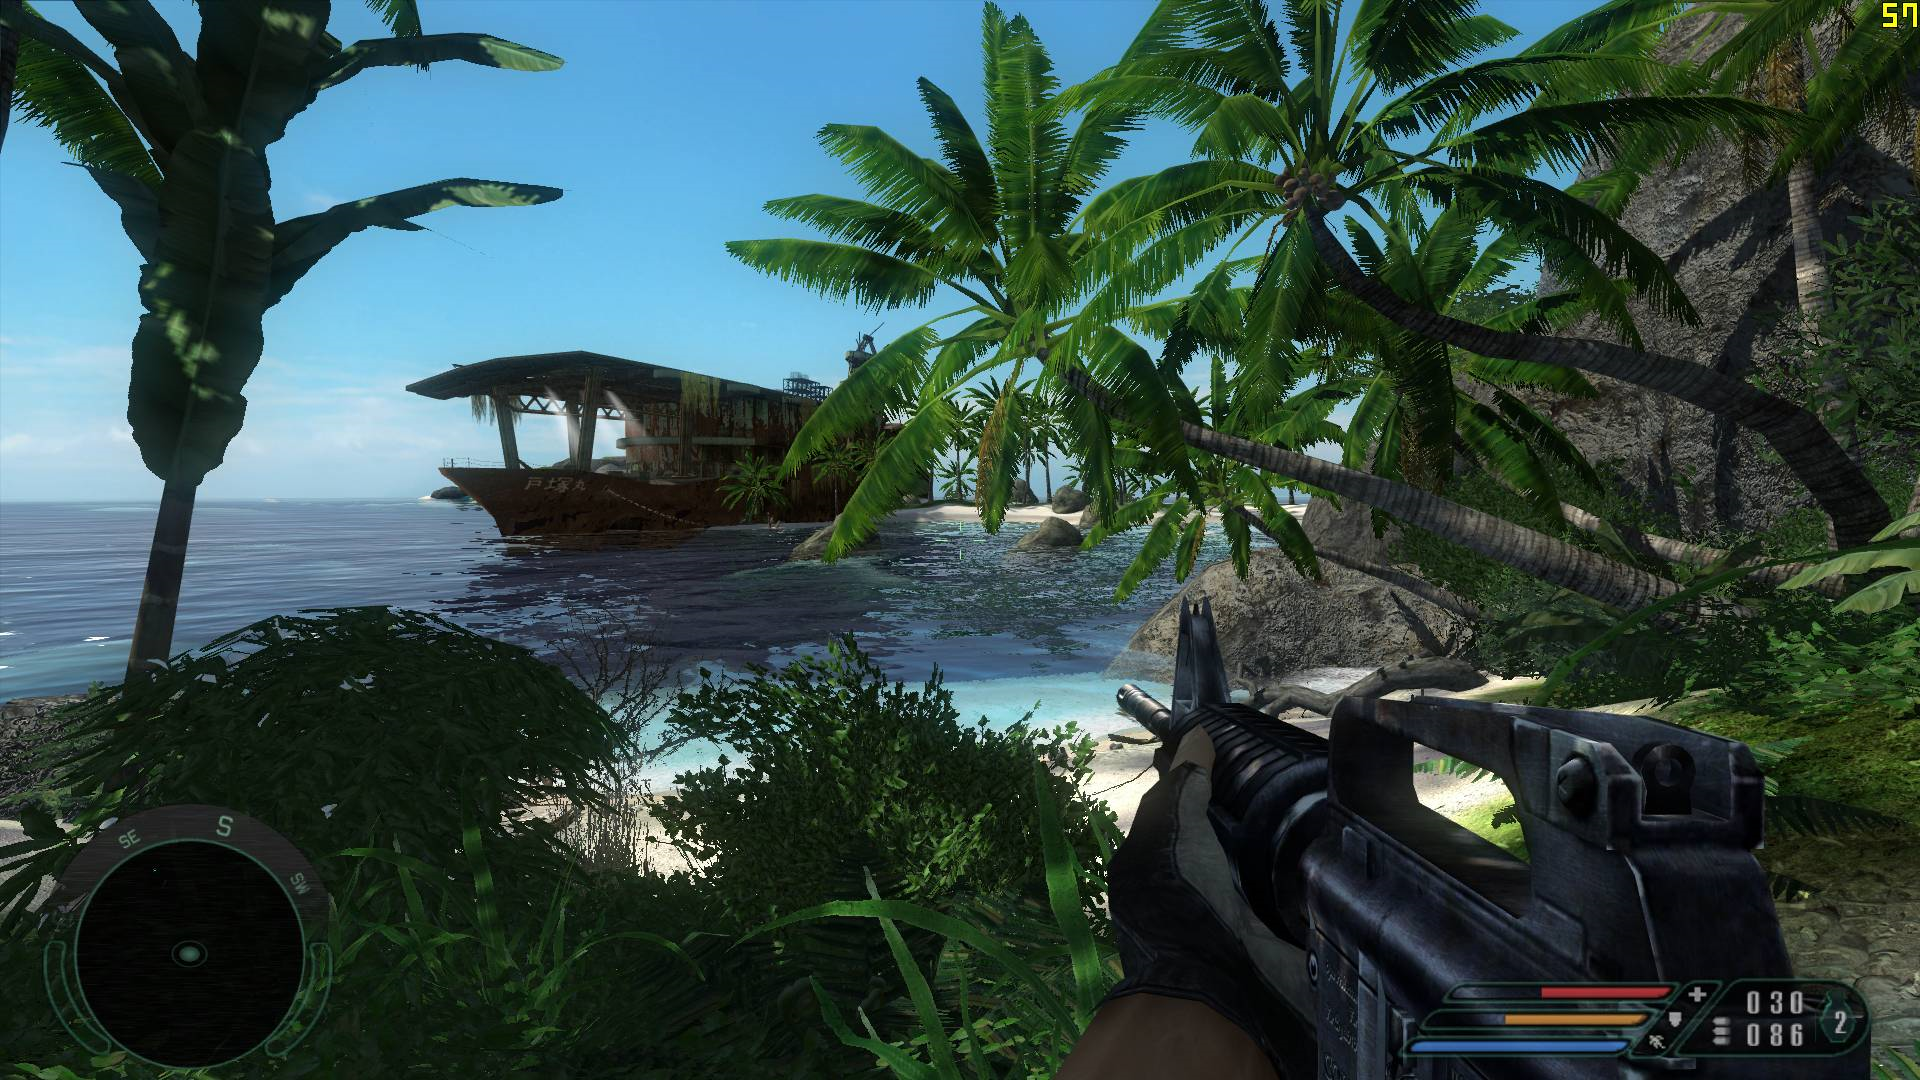
\includegraphics[scale=0.27]{kepek/farcry.png}
\caption{Pillanatkép a Far Cry című játékból (Crytek)}
\label{fig:farcry}
\end{figure}

\section{Egyedi igények és megoldandó problémák}

A saját játékom tervezésekor, megvizsgáltam, hogy milyen jellegű programra, milyen funkciókra van szükség, azt hogyan tervezem majd megvalósítani. Egy kész játékmotor használata helyett egy saját játékmotor implementálására esett a választás. A döntést részben az indokolta, hogy az egyedi funkciók implementálására egy kész játékmotor esetében is szükség lenne. A fő ok viszont az volt, hogy egy játékmotor fejlesztése kimondottan alkalmas különféle matematikával (geometriával, optimalizálással) és programfejlesztéssel (szoftver architektúrával és implementációval)  kapcsolatos problémák vizsgálatára, szemléltetésére és megoldására.

\section{Optimalizálási problémák}

A játékban megvalósítandó elemek között szerepel a lövés, a mesterséges intelligencia, az ütközésvizsgálat, és mindnek megvannak a maga optimalizálási problémái. Ütközésvizsgálatra szükség van a játékos karakterének az ellenfeleknek és a lövéshez is a találatok regisztrálására, pontos helyének számolására. A játéktér háromszögekből áll. A lövés megvalósításához szükségünk van háromszög, és egyenes metszéspontjának számítására, hogy vizualizálható legyen a lövedék becsapódásának helye a talajon, falakon, illetve egyéb játékbeli elemeken. Ez alapjában véve egy matematikai probléma, amit ki kell számoltatni, le kell programozni. Meg kell határozni azt az egyenest, ami azt mutatja meg, éppen merre nézünk, majd vizsgálni kell, hogy az adott egyenes metszi-e a teret alkotó háromszögek egyikét. De mivel több 100000 háromszög és egyenes metszéspontját kellene alap esetben számítani, így ez több optimalizálási problémát is felvet, amit a későbbiekben részletezek.

\section{A játékmotor fő elemei}

\subsection{Mesterséges intelligencia}

% TODO: Itt még nem ilyen, osztály szintjén kellene tárgyalni a dolgot. Az MI és az ütközésvizsgálat kapcsolatát kellene inkább részletezni kicsit.

Az MI osztálynak elsősorban az a feladata, hogy az ellenfelek egy meghatározott útvonalon mozogjanak, ne menjenek át falakon, menjenek egymásba. A véletlenszerűen lerakott ellenfelet a legközelebbi definiált waypoint-hoz kell irányítani, definiálni kell a célpontot (ami elsődlegesen a játékos), és ki kell számítani a pontokon keresztül vezető legrövidebb útvonalat.

\subsection{Hangok}

% TODO: A játékmotorok felsorolása után kellene egy részletesebb leírást csinálni az SDL-ről.

Egy játékhoz hozzátartoznak a hangeffektek, zenék is, amik élvezetessé teszik azt. Egy jól megválasztott zene például nagyon sokat tud javítani a játékélményen. Ezek megszólalásáért az SDL\_mixer felelős, ami lehetővé teszi azt is, hogy több hang egyidőben, átfedésben megszólaljon, és ne várják meg egymást. Ezt a Sound osztályban valósítottam meg. Lehetőség van hangcsatornákat megadni, folyamatos újrajátszást, illetve a hangok egymáshoz viszonyított hangerejét beállítani.

\subsection{Magasságmező}

A játékteret adó domborzat magasságmezővel lett kialakítva. A játék végleges verziójának alap elrendezését, útvonalait határozza meg, az azokon elhelyezkedő díszletek, illetve egyéb objektumok nélkül. Fontos az is, hogy a kép, amelyből a magasságmezőt számolja a program, bárki számára módosítható legyen, képes legyen saját egyedi pályát létrehozni egy egyszerű rajzolóprogram segítségével.

\subsection{Modellek kezelése}

A játéktér domborzatának adatait egy képből, az egyéb modelleket pedig .obj kiterjesztésű fájlból olvassa be a játék. De csak a beolvasás még nem jelenti azt, hogy látjuk is azokat a kijelzőn. Ehhez a VBO-s (Vertex Buffer Object) kirajzolási módszert választottam, ami a videókártyának a legoptimálisabb adatstruktúrában adja át azt a lehető leggyorsabb kirajzoláshoz.

\subsection{A csapda, mint játékelem}

Mindenképp szerettem volna olyan elemet a játékba, ami megkülönbözteti a többi, hasonló, aréna jellegű, túlélős játéktól. Az egyik ilyen elem, hogy ha a játékos egy előre meghatározott időnél több ideig nem mozdul, akkor megjelenik alatta egy csapda, amelybe leesik, és meghal. Vannak olyan játékok, ahol szimplán az ellenfelek ösztönzik a játékost a mozgásra, de a játék itt kikényszeríti azt, hogy a játékosok mozgásban legyenek. A megállásnál a küszöbérték tapasztalati alapon beállítva 5 másodperc lett. Ezt követően megjelenik a csapda modell egy hang kíséretében. Ezt követően 2 másodpercig még a kamera irányát tudja változtatni a játékos, utána viszont már azt sem. Ezt követően az a föld felé fordul, majd értesíti a játékost a történtek okáról.

\subsection{A lövés}

Egy ilyen játékban alapelem az is, hogy tudjunk lőni, mivel e nélkül az egész értelmét vesztené. A játéktér alapvetően egy textúrázott polygonháló. A lövés során azt kell meghatározni, hogy a lövedék melyik háromszögbe ütközne bele, ha a nézet irányába lőnénk, és egyenes pályát feltételeznénk. Ez egy olyan metszéspontszámítást tesz szükségessé, amelyet a játék összes objektumára el kell végeznünk. Megjelenítés szempontjából ez tipikusan egy lövés textúra illesztését jelenti.

% TODO: Az ellenfelekre vonatkozó ütközésvizsgálatnál a hitbox csak addig kell, amíg azt meg sikerül állapítani, hogy a tartalmazó hitbox-ot eltalálta-e a lövés. Azt követően már a konkrét modellre is meg lehet csinálni a vizsgálatot.

\section{A játék szabályai és mechanikája}

Egy belső nézetes lövöldözős játék esetében az adott személy szemszögéből látjuk a virtuális világot. Egy olyan, aréna jellegű, túlélő játékról van szó, amelyben a játékosok mesterséges intelligenciával rendelkező ellenfelekkel (gyakori szóhasználat szerint \textit{bot}-okkal) harcolnak.

A játék során az ellenfelek hullámokban érkeznek. Egy ilyen hullám akkor ér véget, ha a játékosnak megadott számú ellenfelet sikerült eltalálnia. Közben a játékosnak lehetősége van gyógyszert és lőszert szereznie. A játékos teljesítményének függvényében a fegyver fejlesztését is lehetővé teszi a játék.

A klasszikusan felszedhető tárgyak (\textit{powerup}-ok) mellett a játékban, az előzőekhez kinézetükben hasonló csapda jellegű elemek is vannak. A felszedhető elemek hatása így tehát lehet egyaránt pozitív vagy negatív.

A játék megvalósításának problémaköre tehát szerteágazó. Többek között meg kellett valósítani a modellbetöltést textúrázással, az irányítást, fizikát, ütközéskezelést, ellenfelek viselkedésének modellezését, fények és hangok kezelését.

